\documentclass[]{article}
\usepackage[T1]{fontenc}
\usepackage{lmodern}
\usepackage{amssymb,amsmath}
\usepackage{ifxetex,ifluatex}
\usepackage{fixltx2e} % provides \textsubscript
\usepackage{graphicx}
\newcommand{\tab}[1]{\hspace{.2\textwidth}\rlap{#1}}
% use upquote if available, for straight quotes in verbatim environments
\IfFileExists{upquote.sty}{\usepackage{upquote}}{}
\ifnum 0\ifxetex 1\fi\ifluatex 1\fi=0 % if pdftex
  \usepackage[utf8]{inputenc}
\else % if luatex or xelatex
  \ifxetex
    \usepackage{mathspec}
    \usepackage{xltxtra,xunicode}
  \else
    \usepackage{fontspec}
  \fi
  \defaultfontfeatures{Mapping=tex-text,Scale=MatchLowercase}
  \newcommand{\euro}{€}
\fi
% use microtype if available
\IfFileExists{microtype.sty}{\usepackage{microtype}}{}
\def\tightlist{}
\ifxetex
  \usepackage[setpagesize=false, % page size defined by xetex
              unicode=false, % unicode breaks when used with xetex
              xetex]{hyperref}
\else
  \usepackage[unicode=true]{hyperref}
\fi
\hypersetup{breaklinks=true,
            bookmarks=true,
            pdfauthor={Arne Beer MN 6489196; Marta Nevermann MN 6419716; Daniel Waller MN 6813853; Julius Hansen MN 6455291},
            pdftitle={Grundlagen der Wissensverarbeitung -- Tutorial 5, Gruppe 4},
            colorlinks=true,
            citecolor=blue,
            urlcolor=blue,
            linkcolor=magenta,
            pdfborder={0 0 0}}
\urlstyle{same}  % don't use monospace font for urls
\setlength{\parindent}{0pt}
\setlength{\parskip}{6pt plus 2pt minus 1pt}
\setlength{\emergencystretch}{3em}  % prevent overfull lines
\setcounter{secnumdepth}{0}

\title{Grundlagen der Wissensverarbeitung -- Tutorial 5, Gruppe 4}
\author{Arne Beer MN 6489196 \and Marta Nevermann MN 6419716 \and Daniel Waller MN 6813853 \and Julius Hansen MN 6455291}
\date{}

\begin{document}
\maketitle


\subsection{Exercise 1.1}\label{exercise-1.1}

\paragraph{(a)}\label{a}

Variables:
    \begin{itemize}
      \item D,E,M,N,O,R,S,Y,a,b,c,d
    \end{itemize}
Domains:
  \begin{itemize} 
    \item D,E,M,N,O,R,S,Y = \{0,1,2,3,4,5,6,7,8,9\}
    \item a,b,c,d = \{0,1\}
  \end{itemize}

Constraints:
\begin{itemize}
    \item M = 1 
    \item S = 9
    \item $0 \leq D \leq 9$
    \item $0 \leq E \leq 9$
    \item $0 \leq N \leq 9$
    \item $0 \leq O \leq 9$
    \item $0 \leq R \leq 9$
    \item $0 \leq Y \leq 9$
    \item $\forall x : x \neq  x' \leftarrow x \in \{D,E,M,N,O,R,S,Y\} \wedge \ x' \in \{D,E,M,N,O,R,S,Y\}\backslash x$
    \item $D + E = Y * 10a$
    \item $N + R + a = E + 10b$
    \item $E + O + b = N + 10c$
    \item $S + M + c = O + 10d$
    \item $d = M$
\end{itemize}

Die Constraints M = 1 und S = 9 ergeben sich aus dem Aufbau der Gleichung. Wenn gleiche Buchstaben den gleichen Zahlenwert besitzen müssen, dann kann M nur 1 sein und S nur 9, da es keine andere Möglichkeit gibt zwei Tausender ('SEND', 'MORE') so zu addieren, dass unten ein Zehntausender ('MONEY') mit gleicher Anfangsziffer wie der zweite Tausender ('MORE') steht.\newline\newline
Im folgenden constraint network ist domain-consistency gegeben. Alle Arcs, die zu einem Constraint gehören haben die gleiche Farbe.\newline

\begin{figure}[ht]
  \centering
  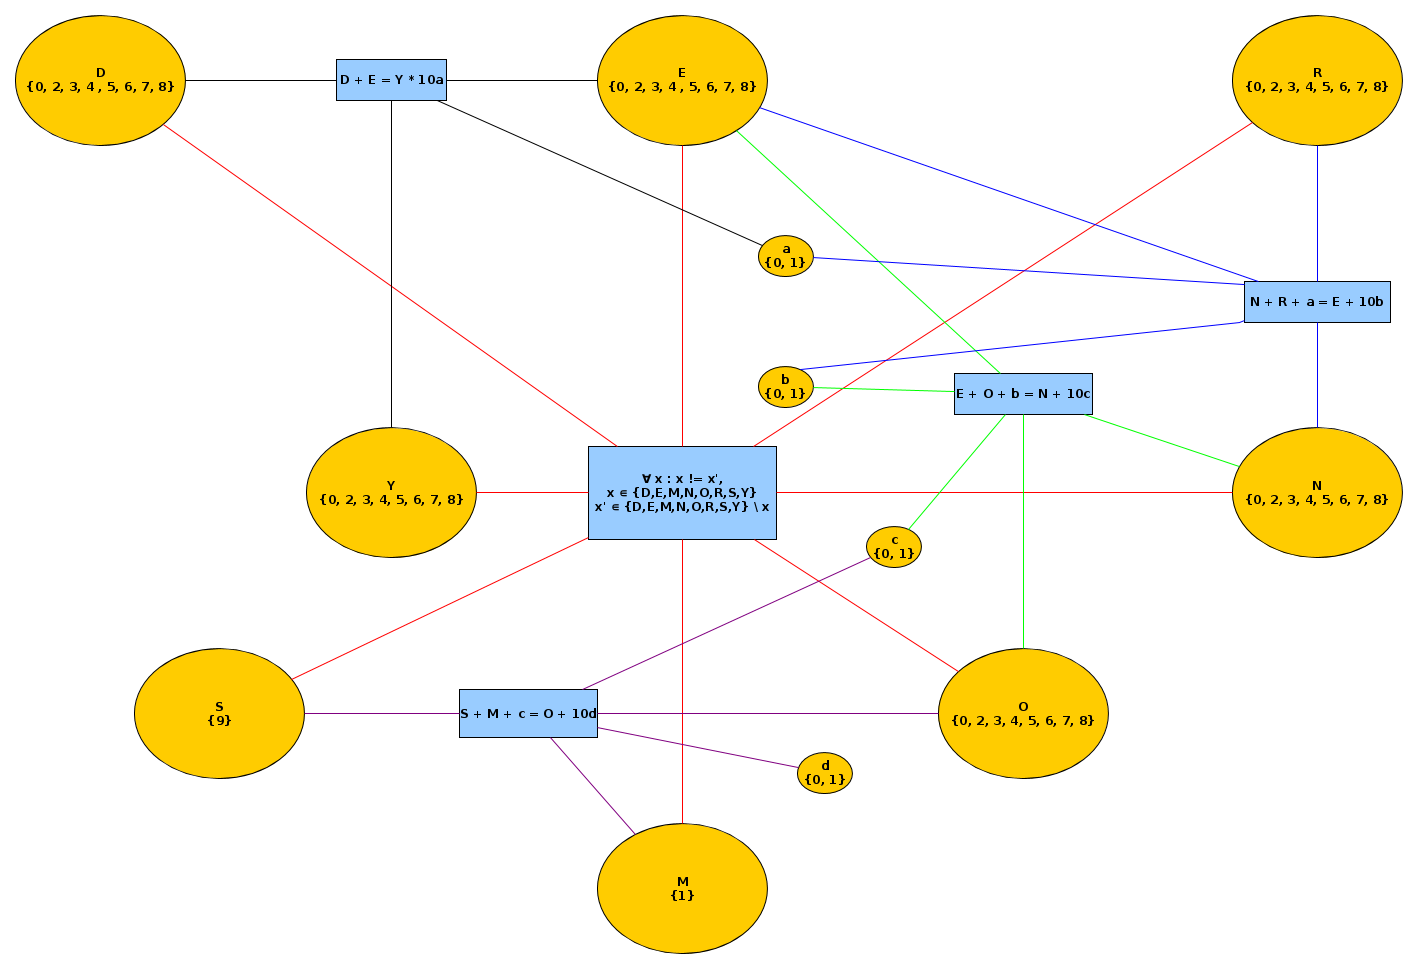
\includegraphics[width=\textwidth]{./constraint_network.png}
\end{figure}

\pagebreak

\paragraph{(b)}\label{b}

Zuerst würden wir versuchen uns anzuschauen, welche Belegungen für das erste vertikale Wort in Frage kommen. Dafür muss gegeben sein, dass alle Buchstaben in dem Wort auch mögliche Anfangsbuchstaben für andere Wörter sind. Also  für $Char_{begin} = \{a,b,e,f,l,o,r,t\}$
\[ Possible_{vert1}  \leftarrow \forall w\in Words : char1_w, char2_w, char3_w \in Char_{begin} \]
Daraus ergeben sich $Possible_{vert1} = \{are, art, bat, bee, boa, ear, eel, eft, far, fat, lee, oaf, rat, tar\}$. 

Als nächstes schaut man sich an, welche Belegungen für das zweite vertikale Wort in Frage kommen. Man muss hierbei beachten, dass der erste Buchstabe sowohl ein möglicher Anfangsbuchstabe sein muss als auch ein möglicher Zweitbuchstabe und dass der letzte Buchstabe sowohl ein möglicher Endbuchstabe als auch ein möglicher Zweitbuchstabe sein muss.\newline
Also für $Char_{middle} = \{a,d,e,f,g,i,n,o,p,r,s,u,w,y\}$ und $Char_{end} = \{a,c,d,e,f,g,h,k,l,m,n,o,r,t\}$
\[ Possible_{vert2} \leftarrow \forall w \in Words : (char1_w \in Char_{start} \cap Char_{middle}) \wedge (char3_w \in Char_{middle} \cap Char_{end}) \]
Hier bekommt man jetzt schon ein paar Probleme, weil es ziemlich unübersichtlich wird und man sich sehr konzentrieren muss und viel auf dem Papier markieren muss, damit man nicht durcheinander kommt.
Es ergeben sich für $Possible_{vert2}$ folgende mögliche Belegungen:\newline
\{add, ado, age, ago, aid, air, and, any, ape, are, awe, aye, ear, far, oaf\}

Für die Belegung der letzten Spalte muss man darauf achten, dass der erste Buchstabe sowohl ein möglicher Anfangsbuchstabe als auch ein möglicher Endbuchstabe sein muss. Der zweite Buchstabe muss dann sowohl ein möglicher Zweitbuchstabe als auch ein möglicher Endbuchstabe sein.\newline
Also für $Char_{begin}$, $Char_{middle}$, $Char_{end}$:
\[ Possible_{vert3} \leftarrow \forall w \in Words : (char1_w \in Char_{start} \cap Char_{end}) \wedge (char2_w \in Char_{middle} \cap Char_{end}) \]
Nach wieder einiger Schreibarbeit und Markiererei bekommt man für $Possible_{vert3}$ folgende Belegungen heraus:\newline
\{add, ado, age, ago, and, any, arc, are, ark, arm, art, aye, ear, eel, eft, far, fat, lee, oaf, rat, tar\}

Nachdem man nun aus den 40 ursprünglichen Wörtern für jede Spalte eine Anzahl an möglichen Belegungen gefunden hat, steht man immer noch vor dem Problem, dass die Lösung nur lokal ist und man nun für alle möglichen Belegungen schauen müsste ob denn auch zulässige Wörter in den Zeilen A1 - A3 dabei heraus kommen. Bei 14 möglichen Belegungen für die erste, 15 möglichen für die zweite und 21 möglichen für die dritte Spalte ist das immer noch ein erheblicher Aufwand, der nicht leicht im Kopf zu bewältigen ist. Eine wesentlich bessere Strategie als stumpfes ausprobieren würde mir auf Anhieb jetzt nicht mehr einfallen.
\pagebreak
\subsection{Exercise 1.2}\label{exercise-1.2}

\end{document}
